\documentclass[../report.tex]{subfiles}
\begin{document}	
	
\chapter{State of the art}
Before developing a \gls{mems} \gls{tpr} for optical waveguides, the integrated passive and active \gls{pr}s found in the recent literature and their underlying concepts are discussed in this chapter. 
			
	\section{Polarization rotator (PR)}	
\gls{pr}s help in rotating polarized fields from one \gls{sop} to another in a controlled manner. Currently, both optical fiber and on-chip based \gls{pr}s are available. 	

	\section{Optical fiber PR}	
In an ordinary (non-polarization-maintaining) fiber, \gls{te} and \gls{tm} have the same nominal phase velocity due to the fiber's circular symmetry. However tiny amounts of random birefringence in such a fiber, or bending in the fiber, will cause a tiny amount of crosstalk from the \gls{tm} to \gls{te} mode or vice versa. And since even a short portion of fiber, over which a tiny coupling coefficient may apply, is many thousands of wavelengths long, even that small coupling between the two polarization modes, applied coherently, can lead to a large power transfer to the \gls{te} or \gls{tm} mode, completely changing the wave's net state of polarization. Since that coupling coefficient was unintended and a result of arbitrary stress or bending applied to fiber, the output state of polarization will itself be random, and will vary as those stresses or bends vary; it will also vary with wavelength.\par

Polarization-maintaining fibers work by intentionally introducing a systematic birefringence in the fiber, so that there are two well defined polarization modes which propagate along the fiber with very distinct phase velocities. The beat length $L_b$ of such a fiber (for a particular wavelength) is the distance (typically a few millimeters) over which the wave in one mode will experience an additional delay of one wavelength compared to the other polarization mode. Thus a length $\dfrac{L_b}{2}$ of such fiber is equivalent to a half-wave plate. Now consider that there might be a random coupling between the two polarization states over a significant length of such fiber. At point 0 along the fiber, the wave in polarization mode 1 induces an amplitude into mode 2 at some phase. However at point $\dfrac{L_b}{2}$ along the fiber, the same coupling coefficient between the polarization modes induces an amplitude into mode 2 which is now $180^\circ$ out of phase with the wave coupled at point zero, leading to cancellation. At point $L_b$ along the fiber the coupling is again in the original phase, but at $\dfrac{3L_b}{2}$ it is again out of phase and so on. The possibility of coherent addition of wave amplitudes through crosstalk over distances much larger than $L_b$ is thus eliminated. Most of the wave's power remains in the original polarization mode, and exits the fiber in that mode's polarization as it is oriented at the fiber end \cite{polarization_maintaining_fiber}. \par	

Electrically driven polarization controller currently available provides a simple, efficient means to manipulate the state of polarization within a singlemode fiber. These operate with negligible insertion and return losses at 100Hz response speed with continuous polarization control capability at low voltage \cite{polarization_maintaining_device}.
		
	\section{On-chip PR}
The currently available \gls{oeic} \gls{pr}s can be classified into two categories as passive and active \gls{pr}s. In the passive \gls{pr}s, the waveguide structures are designed in a specific way to manipulate the effective \gls{ri} of the modes, in order to obtain the desired polarization. The \gls{ri} cannot be manipulated or tuned once fabricated. Whereas, in active \gls{pr}s, the effective \gls{ri} can be actively manipulated by thermo-optic effects, quantum effects or \gls{mems}.
	
		\subsection{Passive PR}
The fields in pure \gls{te} and \gls{tm} modes are orthogonal (i.e. no coupling exists). Thus asymmetric structure in both horizontal and vertical directions are required to break the symmetry, which is accomplished by using different principles viz. mode coupling \cite{dai_novel_2011,ding_Integrated_2013,wang_design_2014}, mode evolution \cite{zhang_selected_2010,chen_compact_2011,zhang_efficient_2012,justin_conference_2012,kazuhiro_integrated_2015} and mode hybridization \cite{fukuda_integrated_2008,leung_numerical_2011,vermeulen_Silicon_2012,velasco_ultracompact_2012}, described in the following sections. All these principles are based on the coupling mode theory described in \ref{concept:mode_coupling}.
			
			\subsubsection{Mode coupling} Mode coupling \gls{pr} includes a pair of waveguides running parallel to each other, with coupled evanescent fields within close proximity. When two modes with orthogonal polarizations have equal effective \gls{ri}s, strong mode coupling occurs in between the waveguides (generally asymmetric directional couplers), and with proper taper orientation and design, length of coupling region, one mode can be effectively converted to the other.
\begin{itemize}[leftmargin=*]
	\item[$\square$] \begin{minipage}[t]{\textwidth}\textbf{Design: Ultra-compact polarization splitter-rotator based on silicon nanowires}
	\begin{figure}[H] %h
		\begin{subfigure}[t]{0.45\textwidth}
			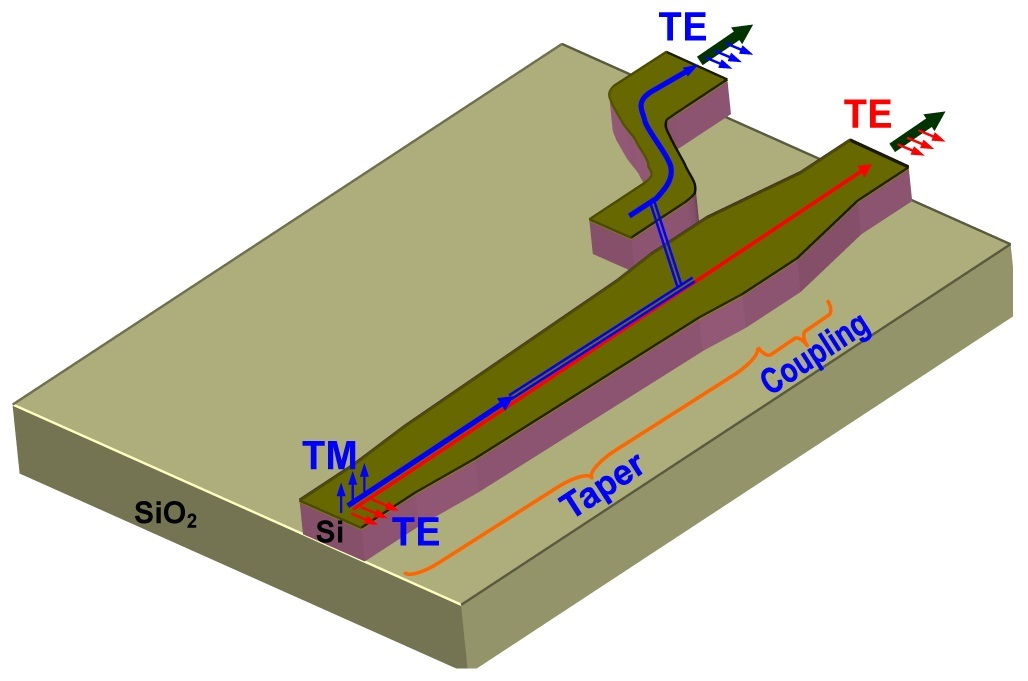
\includegraphics[width=\textwidth]{3-mc-1-1}
			\caption{Structure of the \gls{pr}}
			\label{fig:3_mc_1_1}
		\end{subfigure}
		\hfill
		\begin{subfigure}[t]{0.45\textwidth}
			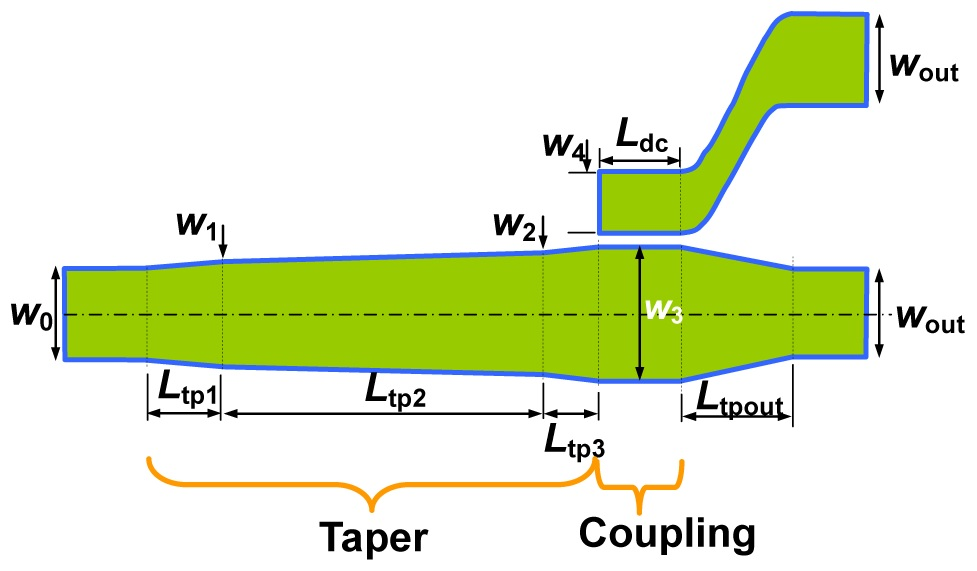
\includegraphics[width=\textwidth]{3-mc-1-2}
			\caption{Schematic of the \gls{pr}}
			\label{fig:3_mc_1_2}
		\end{subfigure}
		\caption{\gls{pr} using mode coupling, by Dai and Bowers \cite{dai_novel_2011}}
	\end{figure}
	\end{minipage}\\\\
	\noindent The coupler (Fig. \ref{fig:3_mc_1_1}) consists of 2 waveguides parallel to each other. The section where coupling occurs is shown in Fig. \ref{fig:3_mc_1_2}. The taper structure is singlemode at the input end ($W_0$) while it becomes multimode at the other end ($W_3$). When light propagates along the taper structure, the \gls{tm} fundamental mode launched at the narrow end ($W_0$) is converted to the first higher-order \gls{te} mode at the wide end ($W_3$) because of the mode coupling between them. Another narrow optical waveguide ($W_4$) is then placed close to the wide waveguide ($W_3$) and an asymmetrical directional coupler is formed. By using this asymmetrical directional coupler, the first higher-order \gls{te} mode in the wide waveguide is then coupled to the \gls{te} fundamental mode of the adjacent narrow waveguide. In this way, the input \gls{tm} fundamental mode at the input waveguide is finally converted into the \gls{te} fundamental mode at the cross port of the asymmetric directional coupler. On the other hand, the input \gls{te} polarization keeps the same polarization state when it goes through the adiabatic taper structure. In the region of the asymmetric directional coupler, the \gls{te} fundamental mode in the wide waveguide could not be coupled to the adjacent narrow waveguide because of the phase mismatching. In this way, \gls{te}- and \gls{tm}- polarized light are separated while the \gls{tm} fundamental mode is also converted into TE fundamental mode \cite{dai_novel_2011}.\par	

	Various other designs for mode coupling have also been proposed \cite{wang_design_2014,ding_Integrated_2013}, which work on the same principle.
	
	\item[$\square$] \textbf{Problem of mode coupling:} The main problem of mode coupling is that directional couplers are not very broadband. Moreover, due to the large birefringence of silicon waveguides, the conversion usually occurs between fundamental \gls{tm} and high order \gls{te} modes and subsequently the high order \gls{te} mode is converted to the fundamental \gls{te} mode.
\end{itemize}		
			\subsubsection{Mode evolution}
The mode evolution based \gls{pr} includes a single waveguide core. The waveguide is designed in such a way that the cross-section of the waveguide varies along the direction of propagation, both in width and height. This changes polarization from \gls{te} to \gls{tm} or vice versa gradually in propagation direction, under adiabatic transition conditions. Since, the cross-section changes gradually and not abruptly, the \gls{per} is high in these type of \gls{pr}s.

\begin{itemize}[leftmargin=*]
	%\item[$\square$] \begin{minipage}[t]{\textwidth}
	\item[$\square$] \begin{minipage}[t]{\textwidth}\textbf{Design A: Mode evolution \gls{pr} based on single taper}
	\begin{figure}[H] %h
		\begin{subfigure}[t]{0.45\textwidth}
			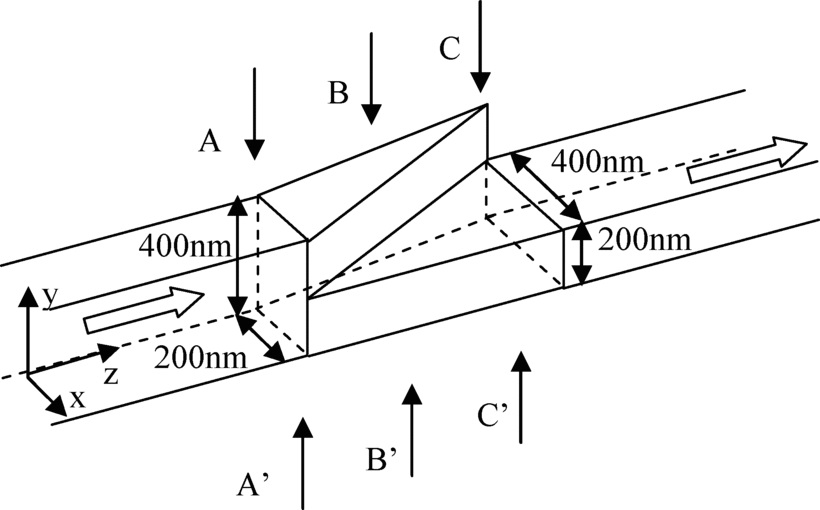
\includegraphics[width=\textwidth]{3-me-2-1}
			\caption{Schematic of the \gls{pr}}
			\label{fig:3_me_2_1}
		\end{subfigure}
		\hfill
		\begin{subfigure}[t]{0.45\textwidth}
			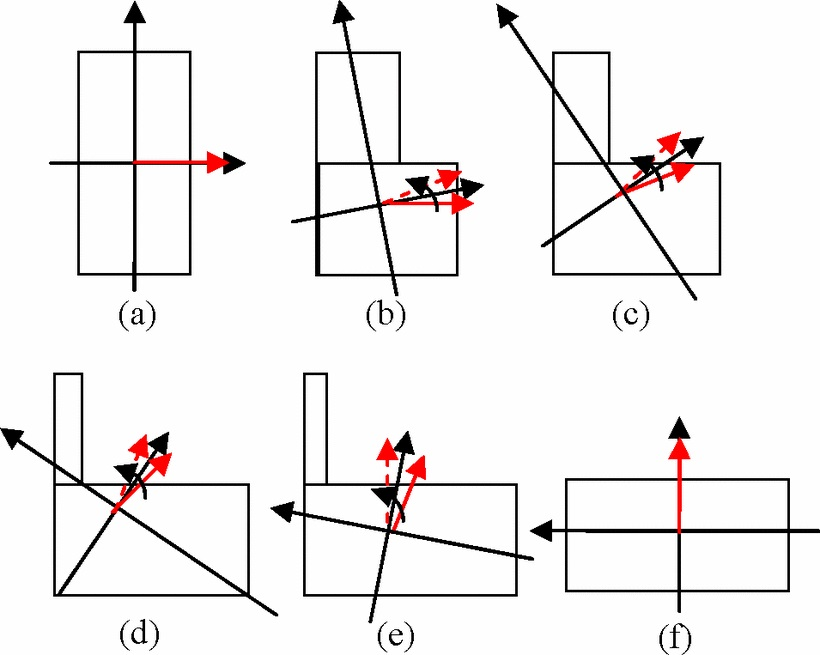
\includegraphics[width=\textwidth]{3-me-2-2}
			\caption{Cross sections of the waveguide at A-A'(a), B-B'(c), and C-C'(f) along with the transition states of the polarization}
			\label{fig:3_me_2_2}
		\end{subfigure}
		\caption{\gls{pr} using mode evolution, by Zhang \textit{et al.} \cite{zhang_selected_2010}}
	\end{figure}
	\end{minipage}\\\\
	\noindent The \gls{pr} (Fig. \ref{fig:3_me_2_1}) consists of the  variable cross section for polarization rotation. The transition region of the rotator was divided into N sections. Each section was considered as a uniform asymmetrical waveguide like the rotator in \cite{wang_ultrasmall_2008}. The length of each section was its half-beat length. The half-beat length of the $n^{th}$ section is $L_{\pi }^{n}=\left( \pi  / \left( \beta _{1}^{n} - \beta _{2}^{n}\right) \right)$ , where $\beta ^{n}=\left( 2\pi / \lambda \right) n_{eff}^{n}$ and $\beta _{1}^{n}$ and $\beta _{2}^{n}$ are the propagation constants of the two fundamental modes in the $n^{th}$ section. After propagating in the $n^{th}$ section, the polarization will rotate $2\Delta \varphi _{n}$ toward the optical axis, where $\varphi _{n}$ is the angle between the optical axis and the polarization of the incident light. The overall rotator should satisfy $\sum _{n}2\Delta \varphi _{n}=90^{0}$, to achieve a rotation of $90^{0}$ in the cascaded sections. Fig. \ref{fig:3_me_2_2} shows the rotation procedure \cite{zhang_selected_2010}.
	%\end{minipage}
			
	\item[$\square$] \begin{minipage}[t]{\textwidth}\textbf{Design B: Mode evolution \gls{pr} composed of an asymmetric-rib waveguide and a tapered waveguide}
	\begin{figure}[H] %h
		\begin{subfigure}[t]{0.45\textwidth}
			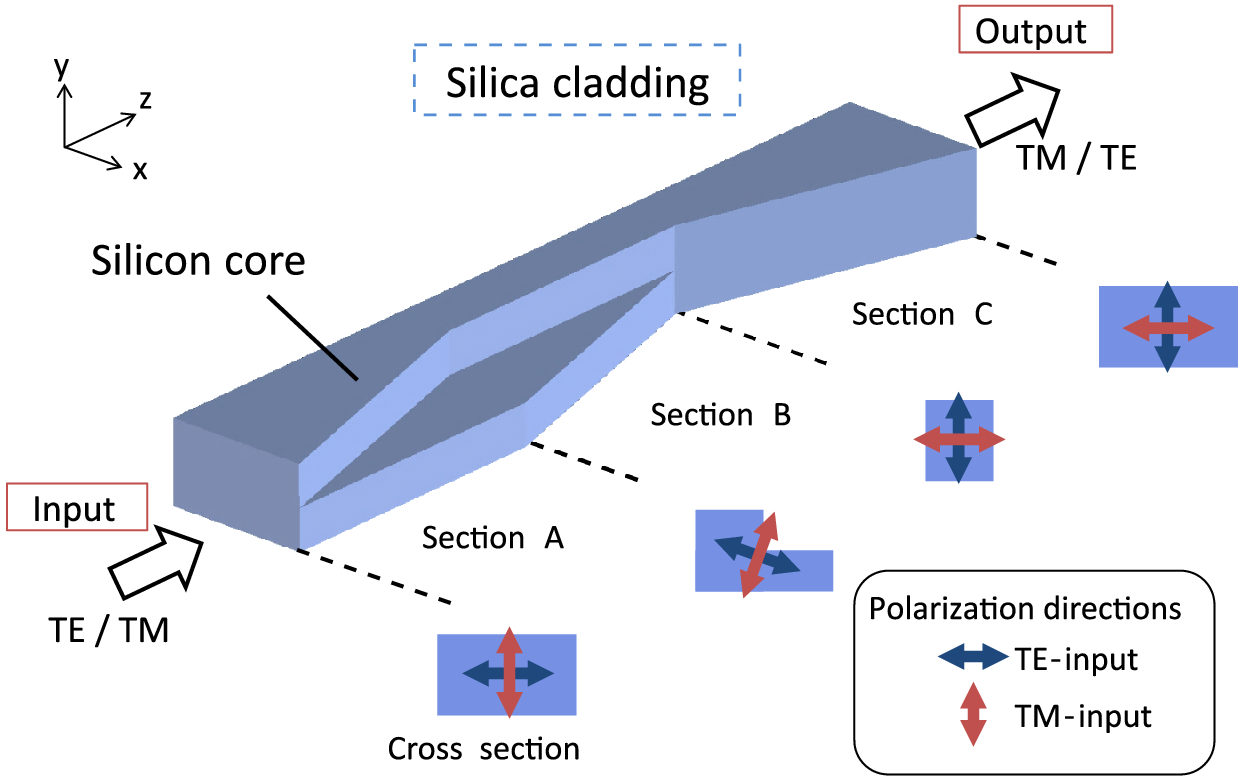
\includegraphics[width=\textwidth]{3-me-1-1}
			\caption{Schematic of the \gls{pr}}
			\label{fig:3_me_1_1}
		\end{subfigure}
		\hfill
		\begin{subfigure}[t]{0.45\textwidth}
			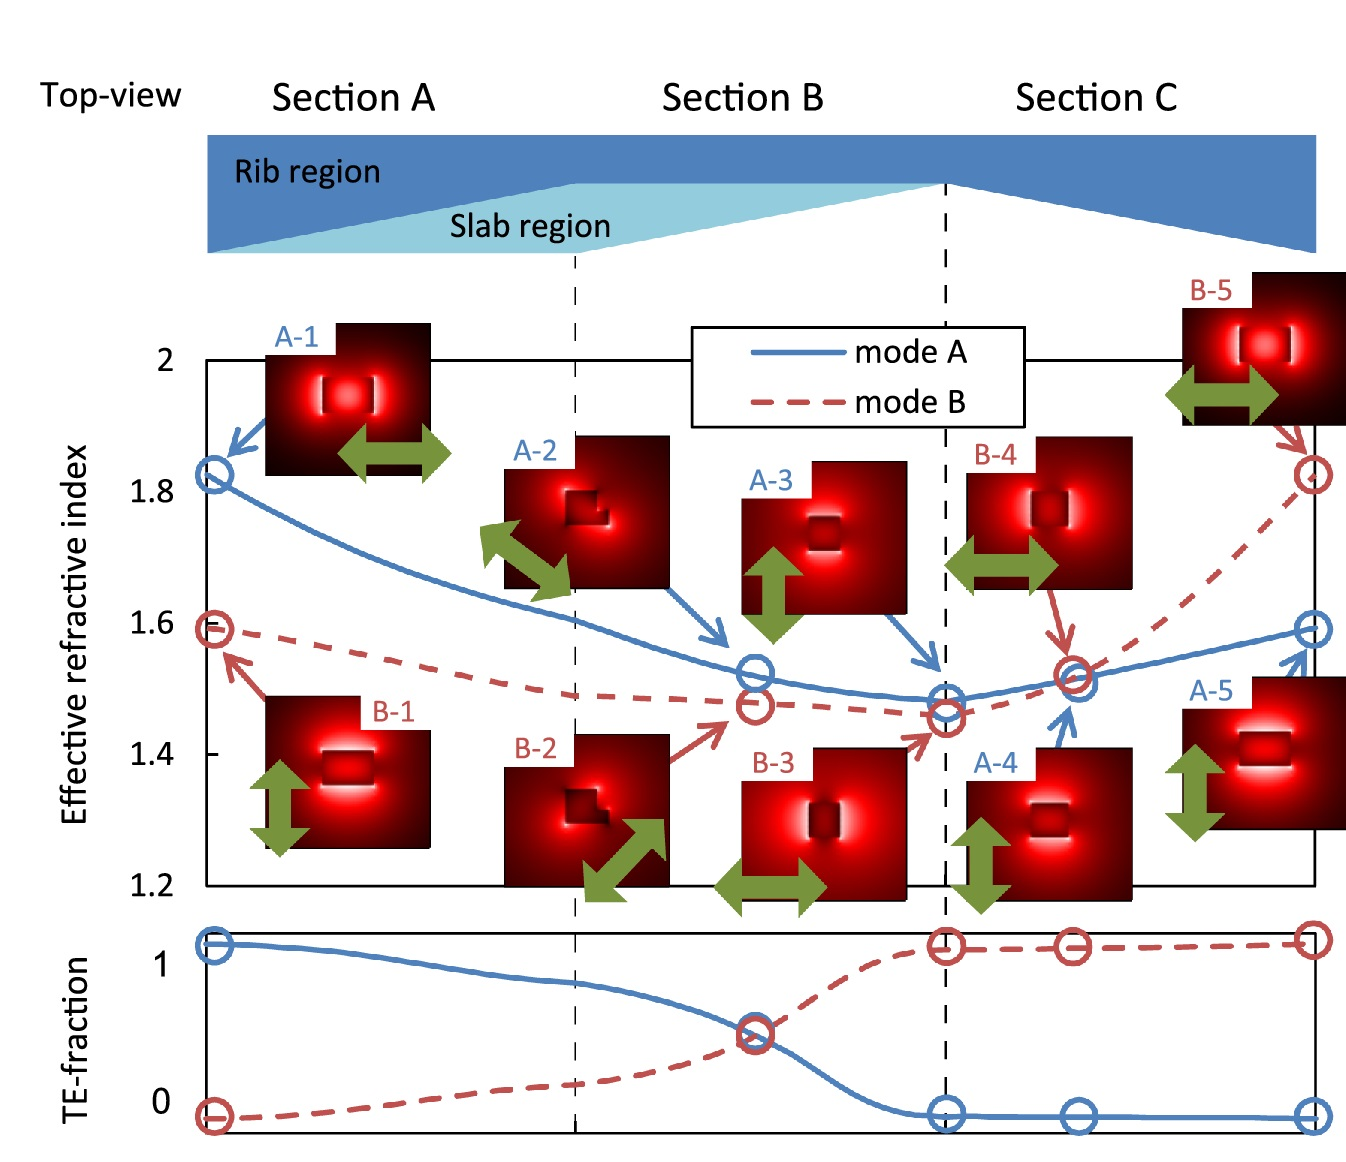
\includegraphics[width=\textwidth]{3-me-1-2}
			\caption{Local mode analysis of the \gls{pr}}
			\label{fig:3_me_1_2}
		\end{subfigure}
		\caption{\gls{pr} using mode evolution, by Goi \textit{et al.} \cite{kazuhiro_integrated_2015}}
	\end{figure}
	\end{minipage}\\\\
	\noindent The \gls{pr} (Fig. \ref{fig:3_me_1_1}) consists of the polarization rotation sections(A and B) with an asymmetric rib waveguide and the mode size conversion section(C) with a nano-tapered waveguide. This design provides both vertical and horizontal asymmetry. \par
	 
	Apart from these, other designs for mode evolution have also been proposed \cite{chen_compact_2011,zhang_efficient_2012,justin_conference_2012}, which has the same basic principle.
	
	\item[$\square$] \textbf{Problem of mode evolution:} In mode evolution, silicon waveguide is specially designed with tapers to enable gradual mode conversion between orthogonal polarization states. Sharp tips at the end of tapers necessary for low conversion loss are also difficult to make. A pure silicon solution is proposed in \cite{zhang_selected_2010}, but in their structure the input and output silicon waveguides have different thicknesses. The structure in \cite{kazuhiro_integrated_2015} solves this problem at the cost of a longer device length of \SI{230}{\micro\meter}. Efficient design of these kind of \gls{pr}s require trade-off between scattering losses at the tapers versus the device length.
\end{itemize}

			\subsubsection{Mode hybridization}
Mode hybridization works by abruptly breaking the symmetry of the silicon waveguide cross section. The propagating modes are hybridized due to introduced asymmetry, allowing optical power to be transferred periodically between the two desired polarization states. The propagation modes excite simultaneously the two fundamental hybrid modes of the asymmetric waveguide, which evolve with different propagation constant. The rotation of $90^{\circ}$ is achieved through interference of the two hybridized modes for a length of $L_{\pi}$, according to the principle of wave plates described mathematically, using \ref{eq:jones_matrix_wp3}. 

\begin{itemize}[leftmargin=*]
	
	\item[$\square$] \begin{minipage}[t]{\textwidth}\textbf{Design A: Asymmetric silicon nanowire waveguide as compact \gls{pr}}
	\begin{figure}[H] %h
		\begin{subfigure}[t]{0.45\textwidth}
			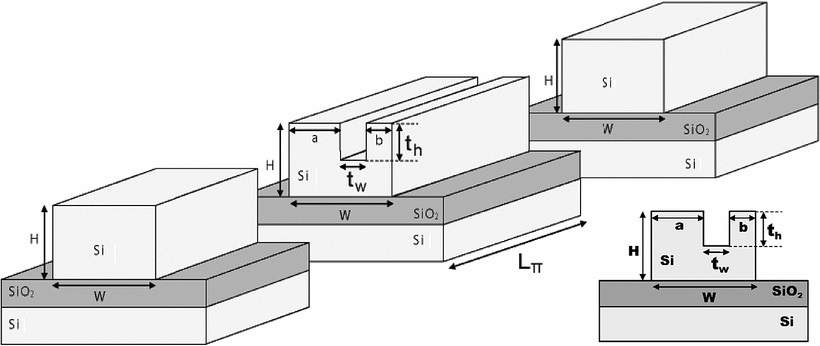
\includegraphics[width=\textwidth]{3-mh-1-1}
			\caption{Schematic diagram of the asymmetric \gls{pr}}
			\label{fig:3_mh_1_1}
		\end{subfigure}
		\hfill
		\begin{subfigure}[t]{0.45\textwidth}
			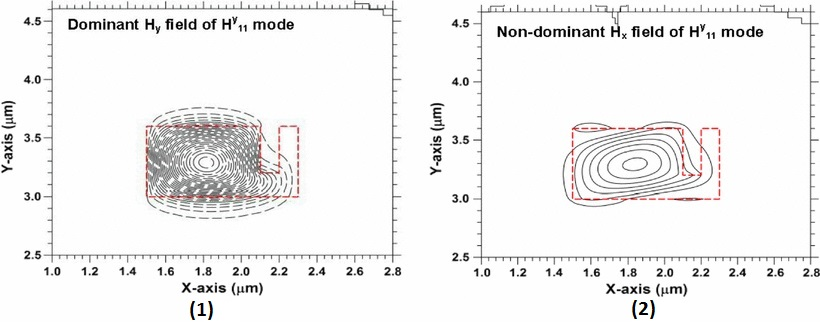
\includegraphics[width=\textwidth]{3-mh-1-2}
			\caption{Contour plots of (1) the dominant $H_y$ field profile and (2) the non-dominant $H_x$ field profile of the $H_{11}^{y}$ mode with $W=800 \si{\nano\meter}$ and $H=800 \si{\nano\meter}$, $t_w=100 \si{\nano\meter}$ and $t_h=400 \si{\nano\meter}$}
			\label{fig:3_mh_1_2}
		\end{subfigure}
		\caption{\gls{pr} using mode hybridization, by Leung \textit{et al.} \cite{leung_numerical_2011}}
	\end{figure}
	\end{minipage}\\\\
	Fig. \ref{fig:3_mh_1_1} depicts the single-stage polarization rotator, which consists of two Si strip waveguides with straight sidewalls, where both are butt coupled to an Si asymmetric strip polarization rotator waveguide in the middle. In the design of a polarization rotator, an asymmetric section which supports the highly hybrid modes is sandwiched between two standard Si waveguides. When a quasi-\gls{te} (or quasi-\gls{tm}) mode from a standard Si waveguide with its polarization angle at nearly zero degrees (or $90^{\circ}$) is launched into the asymmetric section (which supports highly hybrid modes with polarization direction $\pm 45^{\circ }$), then both of them are excited almost equally to satisfy the continuity of the $E_t$ and $H_t$ fields at that interface. These two highly hybrid modes travel along the asymmetric sections. The half-beat length is a key parameter used in order to identify the optimum length of this asymmetrical section to achieve the maximum polarization rotation. The half-beat length is defined as $L_{\pi }= \pi / \Delta \beta$, where $\Delta \beta$ is the difference between the propagation constants of the two hybrid modes. After propagating a distance $L = L_{\pi}$, the original phase condition between the highly polarized modes would be reversed, and the polarization state of the superimposed modes would be rotated by $90^{\circ}$. If a standard Si waveguide (with smaller modal hybridness) is placed at this position, this quasi-\gls{tm} (or quasi-\gls{te}) mode would propagate without any further polarization rotation \cite{leung_numerical_2011}.
	
	\item[$\square$] \textbf{Design B: Efficient silicon \gls{pr} based on mode-hybridization in a double-stair waveguide}\\
	Due to the sudden abruptness introduced in the previous design (Design A) of mode hybridization, the \gls{per} was low. Hence, the abruptness is introduced more gradually in the design, as shown in Fig. \ref{fig:3_mh_2_2}. The design looks like two successive stairs and hence it is called double-stair waveguide. The \gls{pr} \cite{xie_efficient_2015}, based on a double-stair silicon waveguide fabricated with three etch steps as described in Fig.\ref{fig:3_mh_2_1} is better compared to the two-etch-step structure with single-stair cross section \cite{aamer_cmos_2012} because of the higher \gls{per} and broader optical bandwidth achieved. 
	\begin{figure}[H] %h
		\begin{subfigure}[t]{0.45\textwidth}
			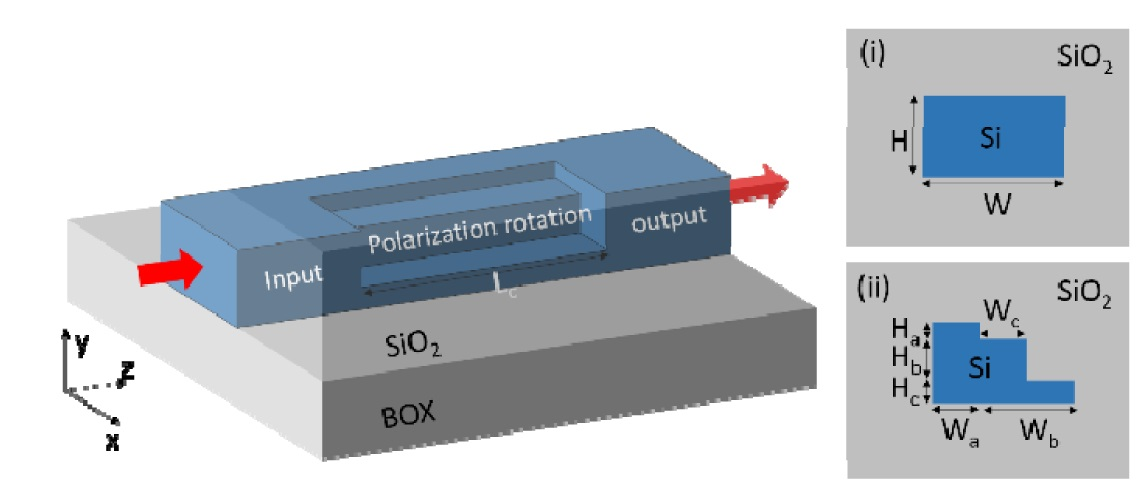
\includegraphics[width=\textwidth]{3-mh-2-1}
			\caption{Schematic structure of the double-stair \gls{pr}. Inset shows the cross-section}
			\label{fig:3_mh_2_1}
		\end{subfigure}
		\hfill
		\begin{subfigure}[t]{0.45\textwidth}
			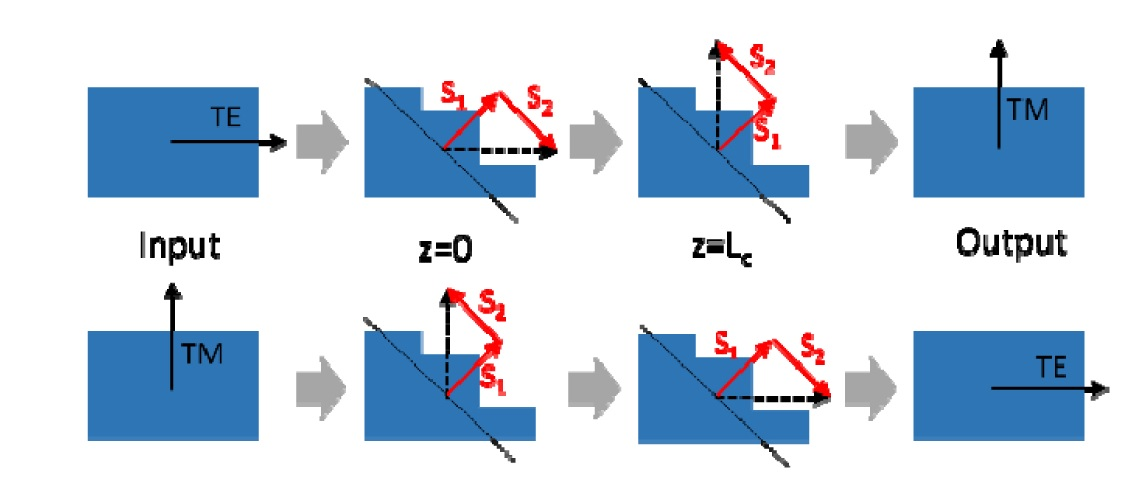
\includegraphics[width=\textwidth]{3-mh-2-2}
			\caption{Polarization rotation process along the waveguide. The arrows indicate the direction of mode electric field. $Z = 0$ is the starting position of the polarization rotation section}
			\label{fig:3_mh_2_2}
		\end{subfigure}
		\caption{\gls{pr} using double-stair waveguide mode hybridization, by Xie \textit{et al.} \cite{xie_efficient_2015}}
	\end{figure}
	\noindent The schematics of the \gls{pr} (Fig. \ref{fig:3_mh_2_1}) consists of the polarization rotation sections and describes the mode conversion along the waveguide.\par
	
	Other designs for mode hybridization have also been proposed \cite{fukuda_integrated_2008,vermeulen_Silicon_2012}, which work on the same principle.
	
	\item[$\square$] \textbf{Problem of mode hybridization:} The narrow trenches ($\sim$\SI{10}{\nano\meter} wide) required for mode hybridization are difficult to pattern and etch with controllable profiles. Recently, a \gls{pr} \cite{aamer_cmos_2012} is realized on a simple strip waveguide by cutting one upper corner of the waveguide in a two-step etch process following the original idea in \cite{wang_ultrasmall_2008}. The pure silicon solution \cite{aamer_cmos_2012}, without the need of extra materials is attractive, but the measured \gls{per} is relatively low around $\sim$\SI{6}{\deci\bel} within a $\sim$\SI{30}{\nano\meter} bandwidth. Although, the double-stair waveguide \cite{xie_efficient_2015}, offers good results but they exhibit wavelength-dependent loss because its working principle relies on interference.
			
\end{itemize}
		
		\subsection{Active PR}\label{sec:active_pr}
An active \gls{pr} is generally achieved by multiple tunable controllers which gives a good trade-off between integration and performance. 
	\subsubsection{Tunable PR with thermo-optic effect} \label{concept:tpps} The \gls{pr}s mainly change the \gls{per}, whereas the \gls{tpps} control the polarization phase. The \gls{tpps} are implemented using waveguide heaters placed alongside the waveguide to avoid losses due to interaction of the evanescent field with the metal. The intensity of the waveguide heaters are electrically controlled.	
	
	\begin{itemize}[leftmargin=*]
		
		\item[$\square$]\begin{minipage}[t]{\textwidth}\textbf{Design: Tunable \gls{pr} with phase shifters}
		\begin{figure}[H] %h
			\begin{subfigure}[t]{0.45\textwidth}
				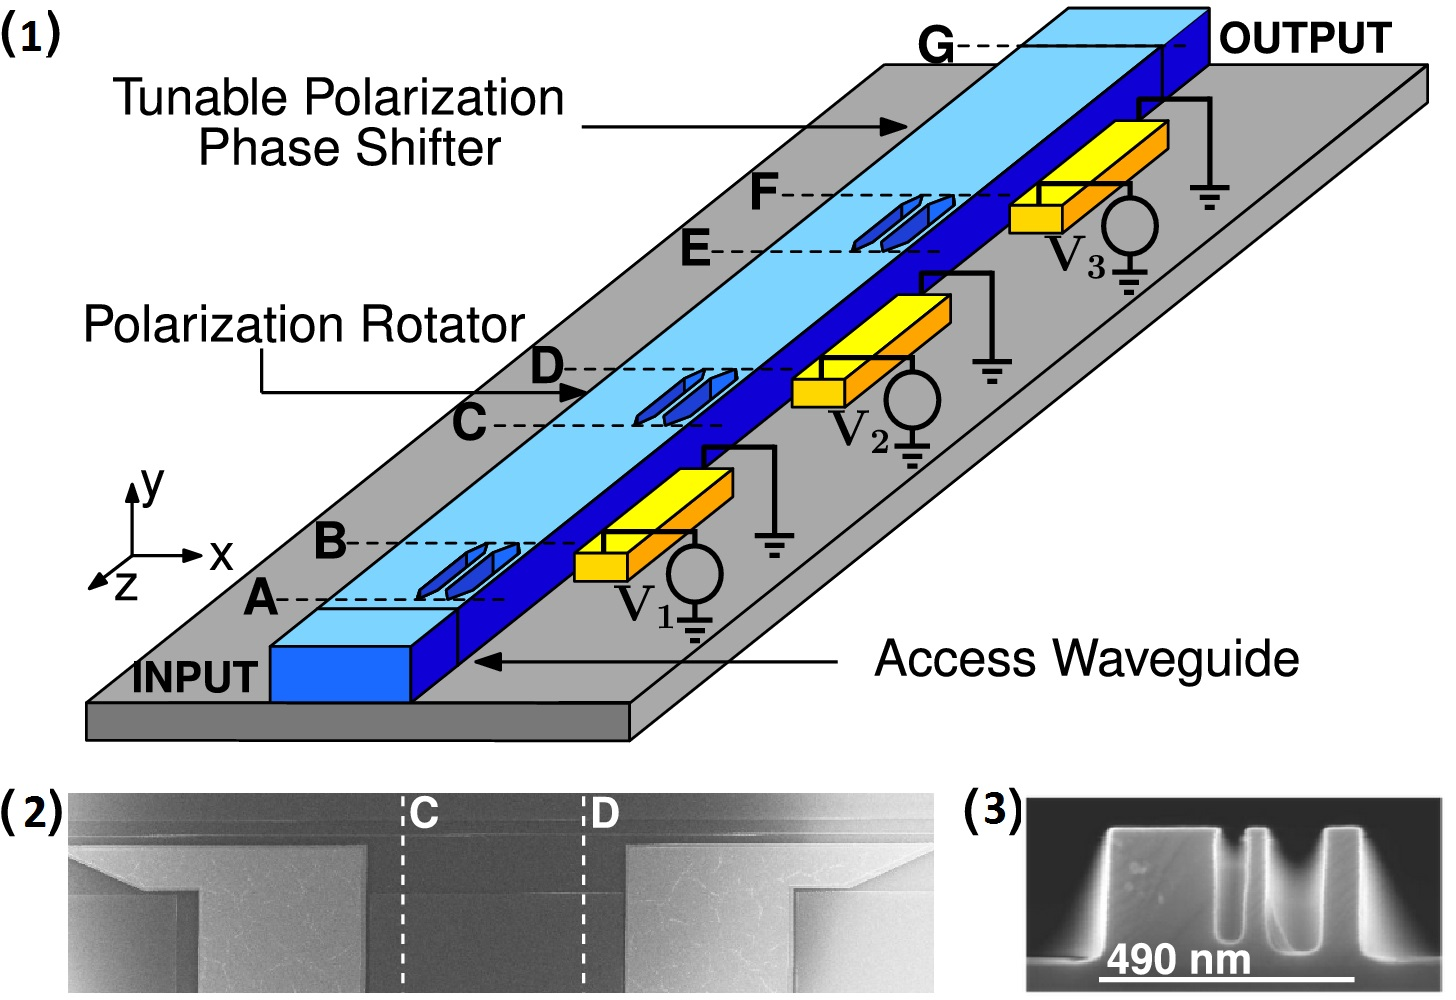
\includegraphics[width=\textwidth]{3-ar-1-1}
				\caption{Schematic of the polarization controller along with the cross section of the \gls{pr}, which uses mode hybridization. The cross section of mode hybridization \gls{pr} can be seen in (3)}
				\label{fig:3_ar_1_1}
			\end{subfigure}
			\hfill
			\begin{subfigure}[t]{0.45\textwidth}
				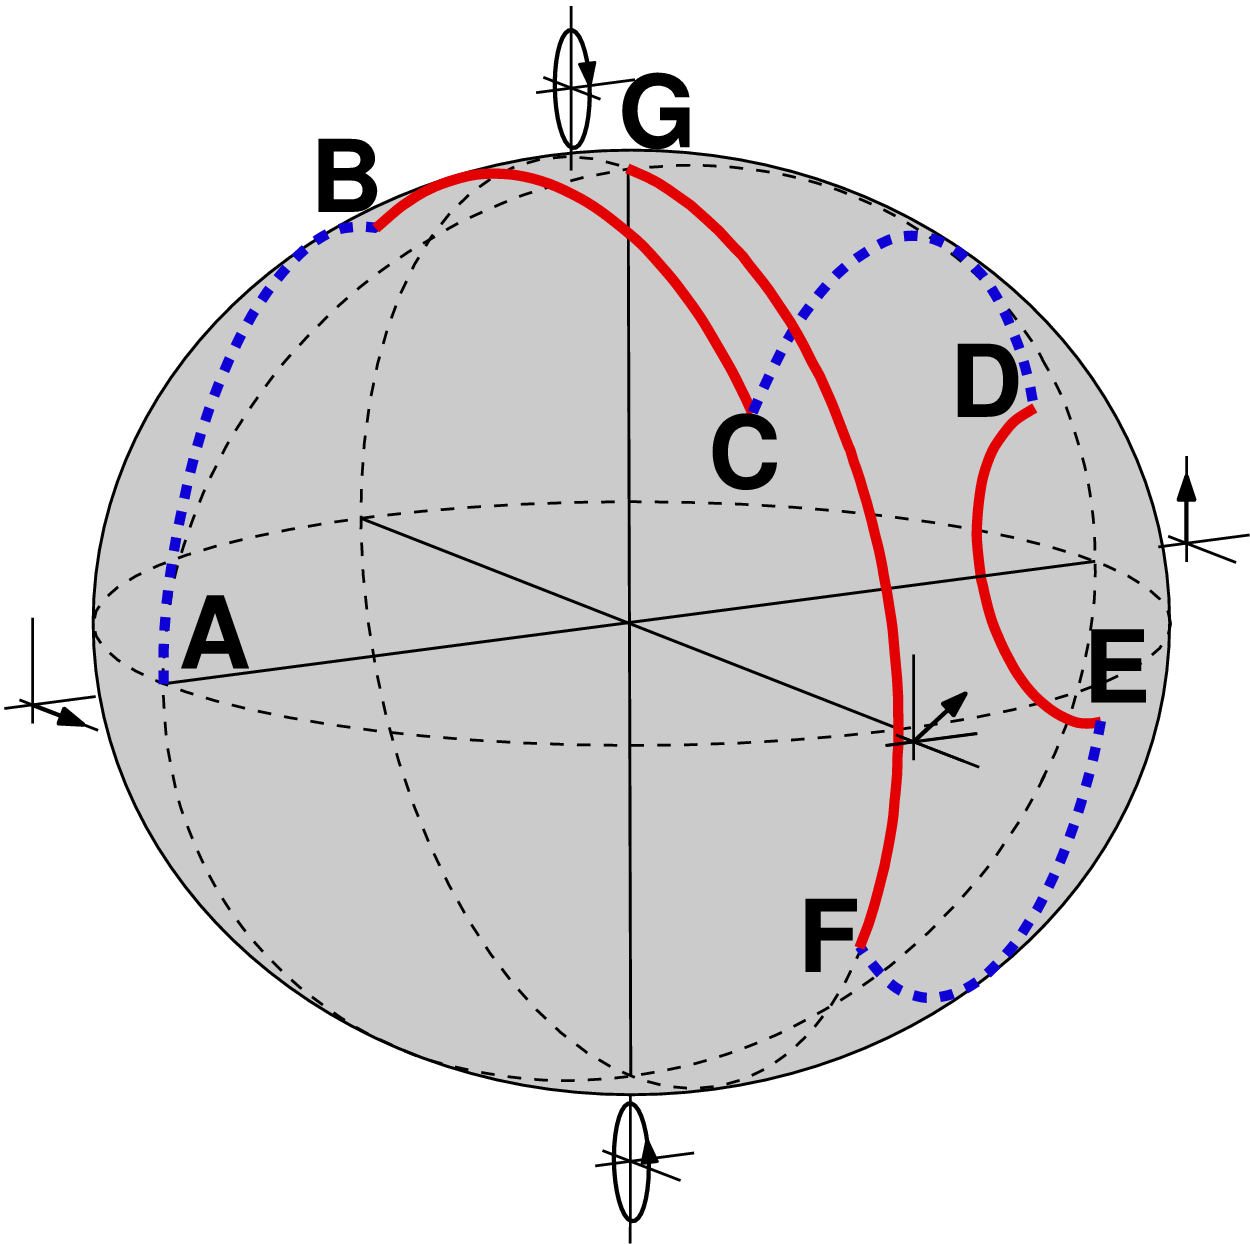
\includegraphics[width=\textwidth]{3-ar-1-2}
				\caption{Evolution of \gls{sop} throughout the device}
				\label{fig:3_ar_1_2}
			\end{subfigure}
			\caption{\gls{pr} control using three \gls{pr} and three \gls{tpps}, by Merenguel \textit{et al.} \cite{sarmiento-merenguel_demonstration_2015}}
		\end{figure}
		\end{minipage}\\\\
		\noindent In the passive \gls{pr}s, the individual \gls{pr} had to produce an exact polarization conversion. This was overcome by the design of the \gls{pr} in Fig. \ref{fig:3_ar_1_1}. The \gls{pr} (Fig. \ref{fig:3_ar_1_1}) consists of three \gls{pr}s and three \gls{tpps} which control the \gls{sop}. The operation of the device is illustrated in Fig. \ref{fig:3_ar_1_2} using the Poincaré sphere \ref{concept:poincare_sphare}. First, a certain \gls{pr} will be performed in the first \gls{pr} (point B). Following the first PR there are two pairs of \gls{tpps}–\gls{pr}. Each \gls{tpps} will tune the polarization phase in order to feed the \gls{pr}s with the suitable polarization phase so that, at the output of the third \gls{pr} (point F), the desired \gls{per} is achieved. The last \gls{tpps} then produces the appropriate polarization phase shift so that the desired \gls{sop} is obtained at the output (point G).
		
		\item[$\square$] \textbf{Drawbacks of PR with thermo-optic effect:}
		Although, the design offers good trade-off between performance and size but still it is limited by the fact that thermal effect can induce phase shift in other waveguides due to cross-talk. This may occur when this system is used in commercial designs with high packing density.
		
		\subsubsection{Tunable PR using Berry's phase} \label{concept:berry_phase} Berry’s phase is a quantum-mechanical phenomenon that may be observed at the macroscopic optical level through the use of an enormous number of photons in a single coherent state \cite{chiao_manifestations_1986}. In the special case of planar (non-helical) paths, such as the paths typically taken by planar optical waveguides, no significant optical rotation is observed independent of the complexity of the path \cite{tomita_observation_1986}. The key to manifest Berry’s phase in photonic integrated circuits is to introduce out-of-plane three-dimensional waveguides to create a two-dimensional momentum space with non-zero (Gaussian) curvature.
		%\subsubsection{Comparative analysis of available PR}
		
	\end{itemize}
	
	\begin{itemize}[leftmargin=*]
		
		\item[$\square$]\begin{minipage}[t]{\textwidth}\textbf{Design: Tunable \gls{pr} with Berry's phase}
			\begin{figure}[H] %h
				\begin{subfigure}[t]{0.33\textwidth}
					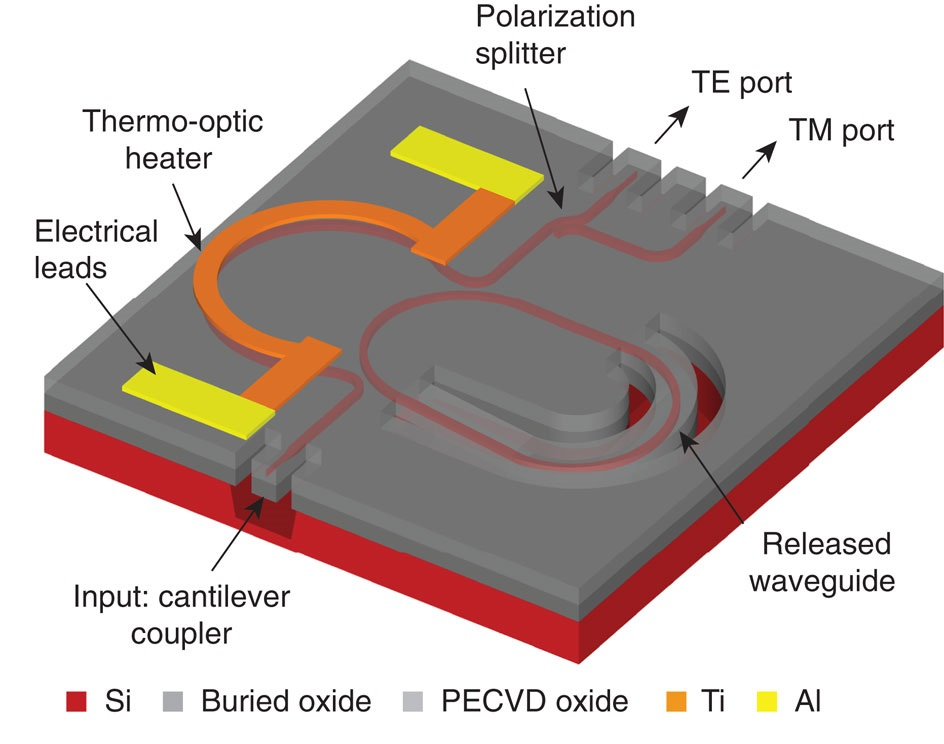
\includegraphics[width=\textwidth]{3-ar-2-1}
					\caption{Schematic of the device}
					\label{fig:3_ar_2_1}
				\end{subfigure}
				\hfill
				\begin{subfigure}[t]{0.33\textwidth}
					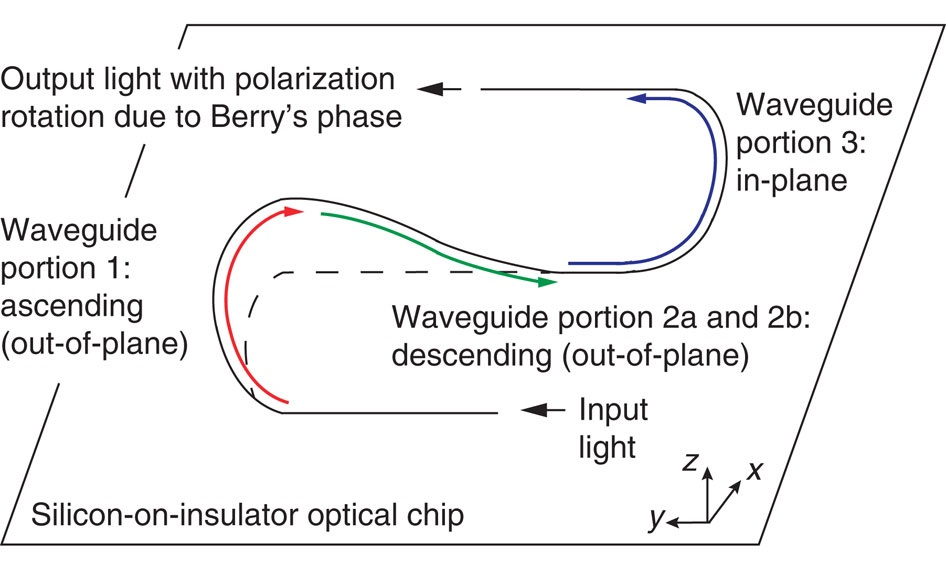
\includegraphics[width=\textwidth]{3-ar-2-2}
					\caption{Layout of device involving out-of-plane waveguides}
					\label{fig:3_ar_2_2}
				\end{subfigure}
				\hfill
				\begin{subfigure}[t]{0.27\textwidth}
					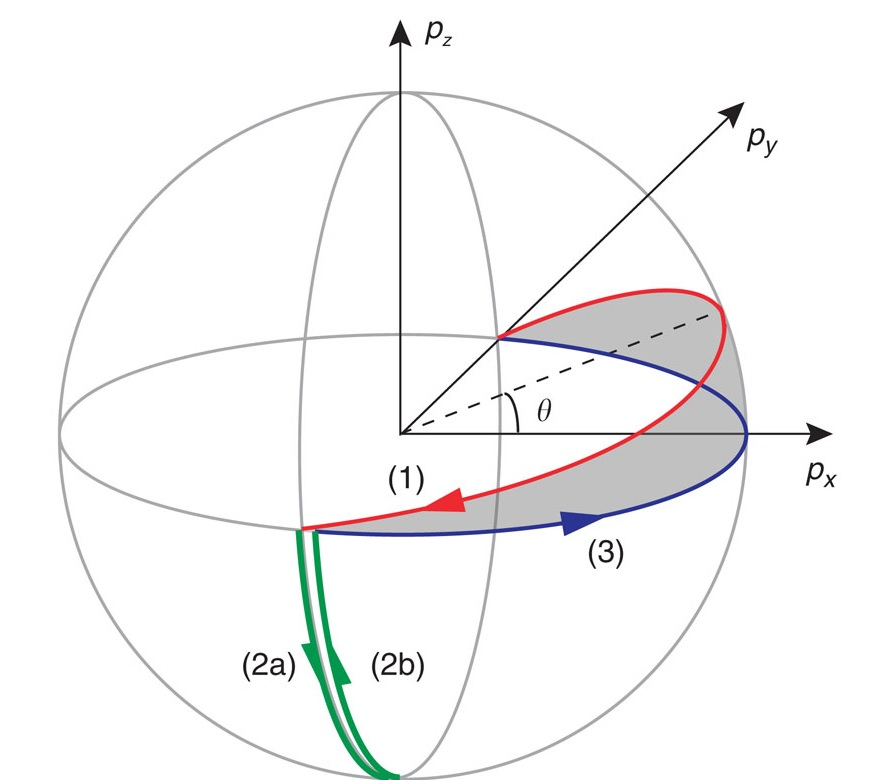
\includegraphics[width=\textwidth]{3-ar-2-3}
					\caption{Evolution of \gls{sop} throughout the device}
					\label{fig:3_ar_2_3}
				\end{subfigure}
				\caption{\gls{pr} control using three \gls{pr} and three \gls{tpps}, by Xu \textit{et al.} \cite{xu_electrically_2014}}
			\end{figure}
		\end{minipage}\\\\
		\noindent Monochromatic light at wavelength $\lambda$ carries a momentum given by $p = p_{x}\widehat {x}+p_{y}\widehat {y}+p_{z}\widehat {z} = \hbar k$, where $k$ is the propagation vector, with magnitude $2\pi/\lambda$ and $\hbar$ is the Planck’s constant divided by $2\pi$. In physical space, the layout consists of three main portions. The first portion, shown in red in Fig. \ref{fig:3_ar_2_2}, consists of an ascending out-of-plane $180^{\circ}$ waveguide bend. The second portion, shown in green, consists of an out-of-plane waveguide that descends to the chip surface. Finally, the third portion consists of an in-plane $180^{\circ}$ bend. In momentum space, the corresponding paths for each waveguide portion are shown in Fig. \ref{fig:3_ar_2_3} using Poincaré sphere (\ref{concept:poincare_sphare}). Light propagation along the three-dimensional path in physical space results in a non-zero subtended solid angle in momentum space, shown as the shaded area in Fig. \ref{fig:3_ar_2_3}. Therefore, the waveguide geometry will exhibit Berry’s phase. A change in wavelength results in a change of the radius of the sphere in momentum space but not the solid angle. If the deflection angle of waveguide portion 1, in the physical space shown in Fig. \ref{fig:3_ar_2_2} is $\theta$, then the output light will appear with polarization rotation equal to $2\theta$ due to Berry’s phase because the magnitude of the solid angle extended by the grey area in momentum space, shown in Fig. \ref{fig:3_ar_2_3}, is $\theta$ \cite{xu_electrically_2014}.
		
		\item[$\square$] \textbf{Drawbacks of PR using Berry's phase:}
		This device uses out-of-plane ring cavity which uses the principles of ring resonator. The ring resonator is limited by its narrow band spectral features which limits bandwidth. Also, the device uses a non-birefringent waveguide, which is lossy in terms of photonic substrate, as an oxide cladding is used to confine light. 	
	\end{itemize}
	
\subsubsection{MEMS tuning}  \gls{mems} is the technology of microscopic devices, particularly those with moving parts on applying voltage. \gls{mems} tuning refers to the integration of \gls{mems} with photonic devices. When applied to micro-resonators, the evanescent field of the resonant mode can be externally perturbed, either from the top or from the sides. Two effects may result as a consequence of such perturbation: change in the effective index of refraction of the mode inside the resonator (since the evanescent tail of the mode sees a different cladding), and increase in the optical loss due to coupling/absorption of the propagating mode into/by the perturbing structure. Coupling ratios between bus waveguides and micro-resonators can also be modified through mechanical movement of suspended bus waveguides, normally needed for post-fabrication tuning or trimming \cite{elfadel_3d_2016}. Opto-mechanical tuning by electrostatic actuation can potentially provide a broad wavelength tuning range, while requiring low energy for operation.

\end{document}
